%% bare_conf.tex
%% V1.4b
%% 2015/08/26
%% by Michael Shell
%% See:
%% http://www.michaelshell.org/
%% for current contact information.
%%
%% This is a skeleton file demonstrating the use of IEEEtran.cls
%% (requires IEEEtran.cls version 1.8b or later) with an IEEE
%% conference paper.
%%
%% Support sites:
%% http://www.michaelshell.org/tex/ieeetran/
%% http://www.ctan.org/pkg/ieeetran
%% and
%% http://www.ieee.org/

%%*************************************************************************
%% Legal Notice:
%% This code is offered as-is without any warranty either expressed or
%% implied; without even the implied warranty of MERCHANTABILITY or
%% FITNESS FOR A PARTICULAR PURPOSE! 
%% User assumes all risk.
%% In no event shall the IEEE or any contributor to this code be liable for
%% any damages or losses, including, but not limited to, incidental,
%% consequential, or any other damages, resulting from the use or misuse
%% of any information contained here.
%%
%% All comments are the opinions of their respective authors and are not
%% necessarily endorsed by the IEEE.
%%
%% This work is distributed under the LaTeX Project Public License (LPPL)
%% ( http://www.latex-project.org/ ) version 1.3, and may be freely used,
%% distributed and modified. A copy of the LPPL, version 1.3, is included
%% in the base LaTeX documentation of all distributions of LaTeX released
%% 2003/12/01 or later.
%% Retain all contribution notices and credits.
%% ** Modified files should be clearly indicated as such, including  **
%% ** renaming them and changing author support contact information. **
%%*************************************************************************


% *** Authors should verify (and, if needed, correct) their LaTeX system  ***
% *** with the testflow diagnostic prior to trusting their LaTeX platform ***
% *** with production work. The IEEE's font choices and paper sizes can   ***
% *** trigger bugs that do not appear when using other class files.       ***                          ***
% The testflow support page is at:
% http://www.michaelshell.org/tex/testflow/



\documentclass[conference]{IEEEtran}
\usepackage{graphicx}
\usepackage{stfloats}
% Some Computer Society conferences also require the compsoc mode option,
% but others use the standard conference format.
%
% If IEEEtran.cls has not been installed into the LaTeX system files,
% manually specify the path to it like:
% \documentclass[conference]{../sty/IEEEtran}





% Some very useful LaTeX packages include:
% (uncomment the ones you want to load)


% *** MISC UTILITY PACKAGES ***
%
%\usepackage{ifpdf}
% Heiko Oberdiek's ifpdf.sty is very useful if you need conditional
% compilation based on whether the output is pdf or dvi.
% usage:
% \ifpdf
%   % pdf code
% \else
%   % dvi code
% \fi
% The latest version of ifpdf.sty can be obtained from:
% http://www.ctan.org/pkg/ifpdf
% Also, note that IEEEtran.cls V1.7 and later provides a builtin
% \ifCLASSINFOpdf conditional that works the same way.
% When switching from latex to pdflatex and vice-versa, the compiler may
% have to be run twice to clear warning/error messages.






% *** CITATION PACKAGES ***
%
%\usepackage{cite}
% cite.sty was written by Donald Arseneau
% V1.6 and later of IEEEtran pre-defines the format of the cite.sty package
% \cite{} output to follow that of the IEEE. Loading the cite package will
% result in citation numbers being automatically sorted and properly
% "compressed/ranged". e.g., [1], [9], [2], [7], [5], [6] without using
% cite.sty will become [1], [2], [5]--[7], [9] using cite.sty. cite.sty's
% \cite will automatically add leading space, if needed. Use cite.sty's
% noadjust option (cite.sty V3.8 and later) if you want to turn this off
% such as if a citation ever needs to be enclosed in parenthesis.
% cite.sty is already installed on most LaTeX systems. Be sure and use
% version 5.0 (2009-03-20) and later if using hyperref.sty.
% The latest version can be obtained at:
% http://www.ctan.org/pkg/cite
% The documentation is contained in the cite.sty file itself.






% *** GRAPHICS RELATED PACKAGES ***
%
\ifCLASSINFOpdf
  % \usepackage[pdftex]{graphicx}
  % declare the path(s) where your graphic files are
  % \graphicspath{{../pdf/}{../jpeg/}}
  % and their extensions so you won't have to specify these with
  % every instance of \includegraphics
  % \DeclareGraphicsExtensions{.pdf,.jpeg,.png}
\else
  % or other class option (dvipsone, dvipdf, if not using dvips). graphicx
  % will default to the driver specified in the system graphics.cfg if no
  % driver is specified.
  % \usepackage[dvips]{graphicx}
  % declare the path(s) where your graphic files are
  % \graphicspath{{../eps/}}
  % and their extensions so you won't have to specify these with
  % every instance of \includegraphics
  % \DeclareGraphicsExtensions{.eps}
\fi
% graphicx was written by David Carlisle and Sebastian Rahtz. It is
% required if you want graphics, photos, etc. graphicx.sty is already
% installed on most LaTeX systems. The latest version and documentation
% can be obtained at: 
% http://www.ctan.org/pkg/graphicx
% Another good source of documentation is "Using Imported Graphics in
% LaTeX2e" by Keith Reckdahl which can be found at:
% http://www.ctan.org/pkg/epslatex
%
% latex, and pdflatex in dvi mode, support graphics in encapsulated
% postscript (.eps) format. pdflatex in pdf mode supports graphics
% in .pdf, .jpeg, .png and .mps (metapost) formats. Users should ensure
% that all non-photo figures use a vector format (.eps, .pdf, .mps) and
% not a bitmapped formats (.jpeg, .png). The IEEE frowns on bitmapped formats
% which can result in "jaggedy"/blurry rendering of lines and letters as
% well as large increases in file sizes.
%
% You can find documentation about the pdfTeX application at:
% http://www.tug.org/applications/pdftex





% *** MATH PACKAGES ***
%
%\usepackage{amsmath}
% A popular package from the American Mathematical Society that provides
% many useful and powerful commands for dealing with mathematics.
%
% Note that the amsmath package sets \interdisplaylinepenalty to 10000
% thus preventing page breaks from occurring within multiline equations. Use:
%\interdisplaylinepenalty=2500
% after loading amsmath to restore such page breaks as IEEEtran.cls normally
% does. amsmath.sty is already installed on most LaTeX systems. The latest
% version and documentation can be obtained at:
% http://www.ctan.org/pkg/amsmath





% *** SPECIALIZED LIST PACKAGES ***
%
%\usepackage{algorithmic}
% algorithmic.sty was written by Peter Williams and Rogerio Brito.
% This package provides an algorithmic environment fo describing algorithms.
% You can use the algorithmic environment in-text or within a figure
% environment to provide for a floating algorithm. Do NOT use the algorithm
% floating environment provided by algorithm.sty (by the same authors) or
% algorithm2e.sty (by Christophe Fiorio) as the IEEE does not use dedicated
% algorithm float types and packages that provide these will not provide
% correct IEEE style captions. The latest version and documentation of
% algorithmic.sty can be obtained at:
% http://www.ctan.org/pkg/algorithms
% Also of interest may be the (relatively newer and more customizable)
% algorithmicx.sty package by Szasz Janos:
% http://www.ctan.org/pkg/algorithmicx




% *** ALIGNMENT PACKAGES ***
%
%\usepackage{array}
% Frank Mittelbach's and David Carlisle's array.sty patches and improves
% the standard LaTeX2e array and tabular environments to provide better
% appearance and additional user controls. As the default LaTeX2e table
% generation code is lacking to the point of almost being broken with
% respect to the quality of the end results, all users are strongly
% advised to use an enhanced (at the very least that provided by array.sty)
% set of table tools. array.sty is already installed on most systems. The
% latest version and documentation can be obtained at:
% http://www.ctan.org/pkg/array


% IEEEtran contains the IEEEeqnarray family of commands that can be used to
% generate multiline equations as well as matrices, tables, etc., of high
% quality.




% *** SUBFIGURE PACKAGES ***
%\ifCLASSOPTIONcompsoc
%  \usepackage[caption=false,font=normalsize,labelfont=sf,textfont=sf]{subfig}
%\else
%  \usepackage[caption=false,font=footnotesize]{subfig}
%\fi
% subfig.sty, written by Steven Douglas Cochran, is the modern replacement
% for subfigure.sty, the latter of which is no longer maintained and is
% incompatible with some LaTeX packages including fixltx2e. However,
% subfig.sty requires and automatically loads Axel Sommerfeldt's caption.sty
% which will override IEEEtran.cls' handling of captions and this will result
% in non-IEEE style figure/table captions. To prevent this problem, be sure
% and invoke subfig.sty's "caption=false" package option (available since
% subfig.sty version 1.3, 2005/06/28) as this is will preserve IEEEtran.cls
% handling of captions.
% Note that the Computer Society format requires a larger sans serif font
% than the serif footnote size font used in traditional IEEE formatting
% and thus the need to invoke different subfig.sty package options depending
% on whether compsoc mode has been enabled.
%
% The latest version and documentation of subfig.sty can be obtained at:
% http://www.ctan.org/pkg/subfig




% *** FLOAT PACKAGES ***
%
%\usepackage{fixltx2e}
% fixltx2e, the successor to the earlier fix2col.sty, was written by
% Frank Mittelbach and David Carlisle. This package corrects a few problems
% in the LaTeX2e kernel, the most notable of which is that in current
% LaTeX2e releases, the ordering of single and double column floats is not
% guaranteed to be preserved. Thus, an unpatched LaTeX2e can allow a
% single column figure to be placed prior to an earlier double column
% figure.
% Be aware that LaTeX2e kernels dated 2015 and later have fixltx2e.sty's
% corrections already built into the system in which case a warning will
% be issued if an attempt is made to load fixltx2e.sty as it is no longer
% needed.
% The latest version and documentation can be found at:
% http://www.ctan.org/pkg/fixltx2e


%\usepackage{stfloats}
% stfloats.sty was written by Sigitas Tolusis. This package gives LaTeX2e
% the ability to do double column floats at the bottom of the page as well
% as the top. (e.g., "\begin{figure*}[!b]" is not normally possible in
% LaTeX2e). It also provides a command:
%\fnbelowfloat
% to enable the placement of footnotes below bottom floats (the standard
% LaTeX2e kernel puts them above bottom floats). This is an invasive package
% which rewrites many portions of the LaTeX2e float routines. It may not work
% with other packages that modify the LaTeX2e float routines. The latest
% version and documentation can be obtained at:
% http://www.ctan.org/pkg/stfloats
% Do not use the stfloats baselinefloat ability as the IEEE does not allow
% \baselineskip to stretch. Authors submitting work to the IEEE should note
% that the IEEE rarely uses double column equations and that authors should try
% to avoid such use. Do not be tempted to use the cuted.sty or midfloat.sty
% packages (also by Sigitas Tolusis) as the IEEE does not format its papers in
% such ways.
% Do not attempt to use stfloats with fixltx2e as they are incompatible.
% Instead, use Morten Hogholm'a dblfloatfix which combines the features
% of both fixltx2e and stfloats:
%
% \usepackage{dblfloatfix}
% The latest version can be found at:
% http://www.ctan.org/pkg/dblfloatfix




% *** PDF, URL AND HYPERLINK PACKAGES ***
%
%\usepackage{url}
% url.sty was written by Donald Arseneau. It provides better support for
% handling and breaking URLs. url.sty is already installed on most LaTeX
% systems. The latest version and documentation can be obtained at:
% http://www.ctan.org/pkg/url
% Basically, \url{my_url_here}.




% *** Do not adjust lengths that control margins, column widths, etc. ***
% *** Do not use packages that alter fonts (such as pslatex).         ***
% There should be no need to do such things with IEEEtran.cls V1.6 and later.
% (Unless specifically asked to do so by the journal or conference you plan
% to submit to, of course. )


% correct bad hyphenation here
\hyphenation{op-tical net-works semi-conduc-tor}


\begin{document}
%
% paper title
% Titles are generally capitalized except for words such as a, an, and, as,
% at, but, by, for, in, nor, of, on, or, the, to and up, which are usually
% not capitalized unless they are the first or last word of the title.
% Linebreaks \\ can be used within to get better formatting as desired.
% Do not put math or special symbols in the title.
\title{Cuttlefish: A Library For Building Distributed Neural Networks}


% author names and affiliations
% use a multiple column layout for up to three different
% affiliations
\author{\IEEEauthorblockN{Abu Kamruzzaman\IEEEauthorrefmark{1},
Rania Mohammedameen Almajalid\IEEEauthorrefmark{2}, Yu Hu\IEEEauthorrefmark{3} and
Tereas Nicole Brooks\IEEEauthorrefmark{4}}
\IEEEauthorblockA{Computer Science,
Pace University\\
Pleasantville NY\\
Email: \IEEEauthorrefmark{1}ak91252p@pace.edu,
\IEEEauthorrefmark{2}ra56319p@pace.edu,
\IEEEauthorrefmark{3}Rain0613@hotmail.com,
\IEEEauthorrefmark{4}tb93141n@pace.edu}}
\maketitle

% conference papers do not typically use \thanks and this command
% is locked out in conference mode. If really needed, such as for
% the acknowledgment of grants, issue a \IEEEoverridecommandlockouts
% after \documentclass

% for over three affiliations, or if they all won't fit within the width
% of the page, use this alternative format:
% 
%\author{\IEEEauthorblockN{Michael Shell\IEEEauthorrefmark{1},
%Homer Simpson\IEEEauthorrefmark{2},
%James Kirk\IEEEauthorrefmark{3}, 
%Montgomery Scott\IEEEauthorrefmark{3} and
%Eldon Tyrell\IEEEauthorrefmark{4}}
%\IEEEauthorblockA{\IEEEauthorrefmark{1}School of Electrical and Computer Engineering\\
%Georgia Institute of Technology,
%Atlanta, Georgia 30332--0250\\ Email: see http://www.michaelshell.org/contact.html}
%\IEEEauthorblockA{\IEEEauthorrefmark{2}Twentieth Century Fox, Springfield, USA\\
%Email: homer@thesimpsons.com}
%\IEEEauthorblockA{\IEEEauthorrefmark{3}Starfleet Academy, San Francisco, California 96678-2391\\
%Telephone: (800) 555--1212, Fax: (888) 555--1212}
%\IEEEauthorblockA{\IEEEauthorrefmark{4}Tyrell Inc., 123 Replicant Street, Los Angeles, California 90210--4321}}




% use for special paper notices
%\IEEEspecialpapernotice{(Invited Paper)}




% make the title area
\maketitle

% As a general rule, do not put math, special symbols or citations
% in the abstract
\begin{abstract}
This paper will discuss the implementation of Cuttlefish, a library for building configurable, fault tolerant, distributed neural networks. Cuttlefish is built on top of the Distributed TensorFlow library. It uses Docker containers to represent units or neurons in the a neural network. More specifically each container (neuron) will run as a service that can communicate with other neurons in the network. Our neural network will be a n layered network, implemented and configured to run on Amazon Web Service's Elastic Container Service (ECS).
\end{abstract}

% no keywords




% For peer review papers, you can put extra information on the cover
% page as needed:
% \ifCLASSOPTIONpeerreview
% \begin{center} \bfseries EDICS Category: 3-BBND \end{center}
% \fi
%
% For peerreview papers, this IEEEtran command inserts a page break and
% creates the second title. It will be ignored for other modes.
\IEEEpeerreviewmaketitle



\section{Introduction}
% no \IEEEPARstart
Machine learning and more specifically the use of Neural Networks have many applications in both the research and commercial software. Though most machine learning techniques and algorithms employed today were developed over 20 years ago the rise of cheap, powerful processors (GPUs and CPUs) and higher capacity storage as allowed these techniques and algorithms to be used at scale.

In this paper we will talk about the implementation of Cuttlefish, a library for building configurable, fault tolerant, distributed neural networks. We will discuss the technologies used to implement this library which includes the use of clustered Docker containers, where each container represents a neuron in the network, Distributed TensorFlow and Amazon Web Service's Elastic Container Service (ECS).

% You must have at least 2 lines in the paragraph with the drop letter
% (should never be an issue)

%\hfill mds
% 
%\hfill August 26, 2015

%\subsection{Subsection Heading Here}
%Subsection text here.
%
%
%\subsubsection{Subsubsection Heading Here}
%Subsubsection text here.

\section{Background}
[TODO: Add intro paragraph for this section]\\

\subsubsection{Docker}
Docker is the world's leading software containerization platform. Docker is open source, designed to make it easier to create, deploy, and run distributed applications inside lightweight Linux containers. It provides a way to run applications securely isolated in a container by packaging it and all its dependencies as well as libraries. Docker containers can wrap the software into a self-contained unit with a complete file-system that contains everything needed to run: operating system, code, runtime, system tools, system libraries, and configured system resources ?. etc. By using Docker containers, we can deploy, and back up a workload regardless of environment quickly and easily more than using virtual machines.

Docker allows to change any application dynamically by adding new capabilities and scaling services which makes containers more portable and flexible to use. Docker also has a mechanism for configuring and spinning up containers that should be clustered together or that are dependencies of one another.

One of the Docker advantages is simplified maintenance which means Docker minimize the efforts and risks which associates with application dependencies. The other advantage is increasing developer productivity because it decreases the time that spent setting up 

\subsubsection{TensorFlow}
TensorFlow is essentially a framework for building Deep Learning Neural Networks. It was developed by engineers and researchers working on the Google Brain Team within Google's Machine Intelligence research organization. It is an open source software library for machine learning computation using data flow graphs. Data flow graphs describe mathematical computation with nodes and edges. Each node in the graph represents mathematical operations, while edges represent the relationships between nodes. A computation expressed using TensorFlow can be executed in one or more GPUs or CPUs in a desktop, mobile device, or server with a single API.

The initial open-source release of TensorFlow supports multiple devices (CPUs and GPUs) in a single computer which is called the single-machine or single node implementation, while the distributed version supports multiple devices (CPUs and GPUs) across a cluster of machines.

\subsubsection{Amazon EC2 Container Service (ECS)}
Amazon EC2 Container Service (ECS) is high performance container management service which supports Docker containers through Management Console or Command Line Interface. It is highly scalable and allows applications to run easily on a managed cluster of Amazon Elastic Compute Cloud (Amazon EC2) instances. Amazon ECS enables applications to be scaled without any additional complexity from a single container to thousands of containers across hundreds of instances. Amazon ECS allows launch and stop container-based applications with simple API calls. 

\section{Motivation}
The initial motivation for Cuttlefish was born from the the observation that neural networks at their core are computational graphs and more specifically directed computational graphs, where each neuron in the graph is a single computation unit. This observation coupled with the understanding that in order to train models and make inference of new data presented to these models at scale, in a production environment, requires implementing neural networks in a way that enables us to infinitely scale the execution of the these computation graphs in way that allows us to leverage all available system resources.  

Tasks for training models and performing inference in neural networks are inherently parallelizable. Hence, it should be possible to implement a library that allows users to create a fault tolerant, distributed neural network, using configurable hyperparameters to drive the dynamic creation a directed graph of neurons (a neural network).  To implement this library a means of represent each node in the network physically; as a device or machine where computation execution will take place. We also need a centralized database to store intermediate values for the weight parameters each neuron calculates during model training. Moreover, the neurons in the network would need an efficient mechanism to communicate and pass data from one neuron to another. Lastly, we would need a mechanism to automate configuring and ''spinning up'' a neural network.  Below we briefly discuss the technologies and approaches needed to implement such a library.

\begin{figure*}
  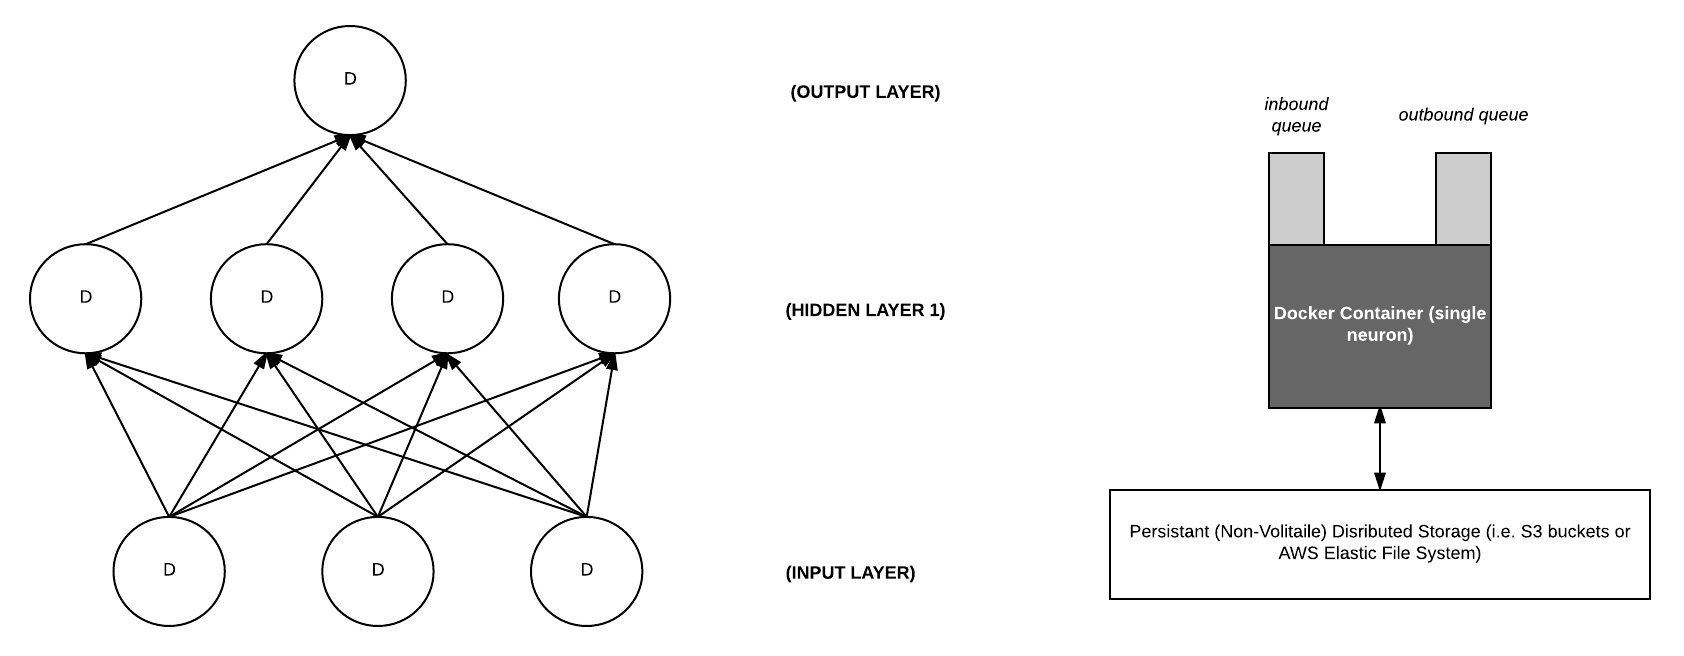
\includegraphics[width=\textwidth]{ml_figure_draft.png}
  \caption{Diagram example neural network nodes as docker containers. Note, the persistent distributed storage represent non-volatile storage for localized data per docker container. Persistent storage is needed to provide fault tolerance for shared and unshared data.}
\end{figure*}

\subsubsection{Physical Representation of Neurons: Docker Containers}
The user of Docker to represent physical a physical neuron was an natural choice because docker containers are self contained units that enable you to provide everything an application would need to run and nothing more; this includes an operating system, file system (volatile file system), and another other needed software, frameworks or tools. Using Docker's Compose tool \cite{docker-compose-doc} containers can easily be configured as dependencies of one another hence allowing you to create a cluster of containers that can be spun up together and can communicate with each other.

\subsubsection{Centralized Storage Of Weighted Model Parameters: Distributed NoSql Database}
For our centralized parameter store, because the data is not highly relational and we would need a scalable solution distributed key, value stores such a Amazon Web Services' DynamoDB would be a good fit.

\subsubsection{Interneuron Communication}
For inter-neural network communication we would need an Inbound and output queue for each neuron in the network in order to pass data such as computed weights, and training model data from node to node. To implement such communication fault tolerant message broker technologies such as rabbitmq \cite{rabbitmq-doc} or Apache Kafka \cite{kafka-doc} are good choices.

\subsubsection{Automation of ''Spinning'' Up Elastic Neural Networks}
Infrastructure orchestration software such as Kubernetes, Mesos and Amazon Web Service's Elastic Container Service are tools used in both test and production environments to automate orchestrations for creating, configuring and managing docker containers, and hence makes them a natural fit for this task.

\section{Our Approach}

** Note, this section should really be called ''Our Proposed Approach'' as is being written before we have implemented Cuttlefish and before we know more about Distributed TensorFlow's capabilities**\\

During the initial research phase of this project, we discovered Google's Distributed TensorFlow project in spirit was very similar the initial idea that motivated our research.  Distributed TensorFlow allows you to create a cluster of servers, where each worker process task is associated a server in the cluster.

Distributed TensorFlow though it is primarily used for modeling machine learning computational models is generic enough to be considered a general purpose distributed computing engine. It offers fault most of the properties we thought were paramount in implementing a library to enable building elastic distributed neural networks: fault  tolerance, a means of sharing common calculated parameters among devices in TensorFlow cluster \cite{dist-tensorflow}, cross device communication, as well as distributed execution of a computation graph among nodes in a TensorFlow cluster.  Hence, we decided to use Distributed TensorFlow as the base for the Culttlefish library.

Note that Cuttlefish defines a docker container as a single server in a TensorFlow cluster. Hence a Cuttlefish distributed neural network is simply defined as TensorFlow cluster.

\subsubsection{Computation Graph Distribution}
TensorFlow uses a greed heuristic algorithm called the ''placement algorithm'' \cite{tensor-flow-white} to determine how a computation graph will be distributed for execution among all available devices. Default supported device types are CPUs and GPUs, there is  also a registration mechanism so that users can implement and register their own device types \cite{tensor-flow-white}. TensorFlow provides an interface for users to influence how the computation graph is distributed, by allowing them to give ''hints and partial constraints'' to the algorithm \cite{tensor-flow-white}. 

Cuttlefish, will use the above described functionality along with the configuration of each docker container?s system resources (memory, number of CPUs etc) to attempt to force TensorFlow?s placement algorithm to map one node in the computation graph to one docker container.  This is will test our the viability of our motivation of using a single docker container to represent a single computational unit in a distributed neural network (neuron).

\subsubsection{Configuring Neural Network (Hyperparameters)}
With Cuttlefish users define the configuration and shape of their neural network?s hyperparameters in a yaml file. By defining these parameters as ''code'', versioning of these parameters is simple, this also allows a user to automate building these configuration files as a tasks in a larger workflow where hyperparameters are being tested for a given set of training data.

\subsubsection{Automation \& Orchestration: Creating Docker Containers As Per Cuttlefish Configuration File}
Cuttlefish?s ''build'' functionality will use the Amazon Web Services' (AWS) elastic contain service?s API \cite{ecs-api} and it's user defined elastic neural network configuration files to configure and build a distributed neural network using a cluster of docker containers (TensorFlow cluster).

With this approach, Cuttlefish takes the paradigm of infrastructure and applies it the configuring and building of a distributed neural network as a cluster of resources readily available for computation tasks.

Note, though we are using AWS' ECS \cite{ecs-doc} for orchestration for this proof of concept, tools like Kubernetes and Mesos are better choice as they offer finder grain control over configuring resource allocation per container. Fine grain control of such resources would allow for configuring and tuning system resources per neuron type, thus making the required system resources fit the computation being performed by a particular neuron. This level of control would be useful when implementing neural networks such as convolutional neural networks, where different types of neurons perform different computational tasks and hence are likely to have different resource needs.

\subsubsection{Data Set}
We are using the MINST data set for training distributed neural networks created by Cuttlefish. ?The MNIST database of handwritten digits, available from this page, has a training set of 60,000 examples, and a test set of 10,000 example.? \cite{mnist-doc} We choice the MINST data set because it is well documented, there is extensive benchmark data for it and TensorFlow as the full data set in a preprocessed ready to use format.


\section{System \& Application Architecture}
TBD

\section{Results}
TBD

\section{Improvements \& Possible Future Work}
TBD

\section{Related Work}
TBD


\section{Conclusion}
TBD

% An example of a floating figure using the graphicx package.
% Note that \label must occur AFTER (or within) \caption.
% For figures, \caption should occur after the \includegraphics.
% Note that IEEEtran v1.7 and later has special internal code that
% is designed to preserve the operation of \label within \caption
% even when the captionsoff option is in effect. However, because
% of issues like this, it may be the safest practice to put all your
% \label just after \caption rather than within \caption{}.
%
% Reminder: the "draftcls" or "draftclsnofoot", not "draft", class
% option should be used if it is desired that the figures are to be
% displayed while in draft mode.
%
%\begin{figure}[!t]
%\centering
%\includegraphics[width=2.5in]{myfigure}
% where an .eps filename suffix will be assumed under latex, 
% and a .pdf suffix will be assumed for pdflatex; or what has been declared
% via \DeclareGraphicsExtensions.
%\caption{Simulation results for the network.}
%\label{fig_sim}
%\end{figure}

% Note that the IEEE typically puts floats only at the top, even when this
% results in a large percentage of a column being occupied by floats.


% An example of a double column floating figure using two subfigures.
% (The subfig.sty package must be loaded for this to work.)
% The subfigure \label commands are set within each subfloat command,
% and the \label for the overall figure must come after \caption.
% \hfil is used as a separator to get equal spacing.
% Watch out that the combined width of all the subfigures on a 
% line do not exceed the text width or a line break will occur.
%
%\begin{figure*}[!t]
%\centering
%\subfloat[Case I]{\includegraphics[width=2.5in]{box}%
%\label{fig_first_case}}
%\hfil
%\subfloat[Case II]{\includegraphics[width=2.5in]{box}%
%\label{fig_second_case}}
%\caption{Simulation results for the network.}
%\label{fig_sim}
%\end{figure*}
%
% Note that often IEEE papers with subfigures do not employ subfigure
% captions (using the optional argument to \subfloat[]), but instead will
% reference/describe all of them (a), (b), etc., within the main caption.
% Be aware that for subfig.sty to generate the (a), (b), etc., subfigure
% labels, the optional argument to \subfloat must be present. If a
% subcaption is not desired, just leave its contents blank,
% e.g., \subfloat[].


% An example of a floating table. Note that, for IEEE style tables, the
% \caption command should come BEFORE the table and, given that table
% captions serve much like titles, are usually capitalized except for words
% such as a, an, and, as, at, but, by, for, in, nor, of, on, or, the, to
% and up, which are usually not capitalized unless they are the first or
% last word of the caption. Table text will default to \footnotesize as
% the IEEE normally uses this smaller font for tables.
% The \label must come after \caption as always.
%
%\begin{table}[!t]
%% increase table row spacing, adjust to taste
%\renewcommand{\arraystretch}{1.3}
% if using array.sty, it might be a good idea to tweak the value of
% \extrarowheight as needed to properly center the text within the cells
%\caption{An Example of a Table}
%\label{table_example}
%\centering
%% Some packages, such as MDW tools, offer better commands for making tables
%% than the plain LaTeX2e tabular which is used here.
%\begin{tabular}{|c||c|}
%\hline
%One & Two\\
%\hline
%Three & Four\\
%\hline
%\end{tabular}
%\end{table}


% Note that the IEEE does not put floats in the very first column
% - or typically anywhere on the first page for that matter. Also,
% in-text middle ("here") positioning is typically not used, but it
% is allowed and encouraged for Computer Society conferences (but
% not Computer Society journals). Most IEEE journals/conferences use
% top floats exclusively. 
% Note that, LaTeX2e, unlike IEEE journals/conferences, places
% footnotes above bottom floats. This can be corrected via the
% \fnbelowfloat command of the stfloats package.



% trigger a \newpage just before the given reference
% number - used to balance the columns on the last page
% adjust value as needed - may need to be readjusted if
% the document is modified later
%\IEEEtriggeratref{8}
% The "triggered" command can be changed if desired:
%\IEEEtriggercmd{\enlargethispage{-5in}}

% references section

% can use a bibliography generated by BibTeX as a .bbl file
% BibTeX documentation can be easily obtained at:
% http://mirror.ctan.org/biblio/bibtex/contrib/doc/
% The IEEEtran BibTeX style support page is at:
% http://www.michaelshell.org/tex/ieeetran/bibtex/
%\bibliographystyle{IEEEtran}
% argument is your BibTeX string definitions and bibliography database(s)
%\bibliography{IEEEabrv,../bib/paper}
%
% <OR> manually copy in the resultant .bbl file
% set second argument of \begin to the number of references
% (used to reserve space for the reference number labels box)

%\begin{thebibliography}{1}
%
%\bibitem{IEEEhowto:kopka}
%H.~Kopka and P.~W. Daly, \emph{A Guide to \LaTeX}, 3rd~ed.\hskip 1em plus
%  0.5em minus 0.4em\relax Harlow, England: Addison-Wesley, 1999.
%
%\end{thebibliography}

\bibliographystyle{plain}
\bibliography{ml_project_draft.bib}



% that's all folks
\end{document}


